% Created 2020-04-26 Sun 11:59
% Intended LaTeX compiler: pdflatex
\documentclass[11pt]{article}
\usepackage[utf8]{inputenc}
\usepackage[T1]{fontenc}
\usepackage{graphicx}
\usepackage{grffile}
\usepackage{longtable}
\usepackage{wrapfig}
\usepackage{rotating}
\usepackage[normalem]{ulem}
\usepackage{amsmath}
\usepackage{textcomp}
\usepackage{amssymb}
\usepackage{capt-of}
\usepackage{hyperref}
\usepackage{/home/ryan/Dropbox/profiles/Templates/LaTeX/ScreenStyle}
\author{Ryan Greenup}
\date{\today}
\title{Scratch Buffer 05 PCA and MDS Visualisation}
\hypersetup{
 pdfauthor={Ryan Greenup},
 pdftitle={Scratch Buffer 05 PCA and MDS Visualisation},
 pdfkeywords={},
 pdfsubject={},
 pdfcreator={Emacs 27.0.91 (Org mode 9.4)}, 
 pdflang={English}}
\begin{document}

\maketitle
\tableofcontents


\section{Visualisation and MDS}
\label{sec:orgdc07b8f}
\subsection{Load Packages}
\label{sec:org03a95a4}
First Load all the packages:

\begin{verbatim}
  # Load Packages -----------------------------------------------------------

    if(require("pacman")){
      library(pacman)
    }else{
      install.packages("pacman")
      library(pacman)
    }
      pacman::p_load(xts, sp, gstat, ggplot2, rmarkdown, reshape2, ggmap,
                   parallel, dplyr, plotly, tidyverse, reticulate, UsingR, Rmpfr,
                   swirl, corrplot, gridExtra, mise, latex2exp, tree, rpart, lattice,
                   coin, primes, epitools, maps, clipr, ggmap, twitteR, ROAuth,
                   tm, rtweet, base64enc, httpuv, SnowballC, RColorBrewer, wordcloud, ggwordcloud)
  mise()
\end{verbatim}

The tokens are located in \texttt{KeePass}:

\begin{verbatim}
  # Set up Tokens ===========================================================

       options(RCurlOptions = list(verbose = FALSE, capath = system.file("CurlSSL", "cacert.pem", package = "RCurl"), ssl.verifypeer = FALSE))

     setup_twitter_oauth(
       consumer_key = "dE7...",
       consumer_secret = "7B...",
       access_token = "1240821...",
       access_secret = "HLBWzHce...")

  # rtweet ==================================================================
  tk <-    rtweet::create_token(
       app = "SWA",
       consumer_key    = "dE7H...",
       consumer_secret = "7By...",
       access_token    = "1240...",
       access_secret   = "HLBWzH...",
       set_renv        = FALSE)
\end{verbatim}

\subsection{Get Tweets}
\label{sec:orgbc51642}
In order to practice visualisation using PCA, it may be helpful to have
data that appears to cluster, so political tweets would be ideal, we can
use the handles for the party leaders:

\begin{verbatim}
  # Political Tweets --------------------------------------------------------
     n <- 100

     # twitteR::userTimeline("billshortemp", n = n)
  altw <- rtweet::get_timeline("AlboMP",   n = n, token = tk)
  smtw <- rtweet::get_timeline("ScottMorrisonMP",       n = n, token = tk)
  abtw <- rtweet::get_timeline("AdamBandt", n = n, token = tk)
\end{verbatim}

\subsubsection{Create a Corpus}
\label{sec:orgb78d988}
The \texttt{tm} package requires tweets to be stored in a \texttt{corpus} object,
there are three steps to creating this: 1. Extract the Text 2. use
\texttt{tm::VectorSource(text)} to create a \texttt{tm} source file. 3. use
\texttt{tm::VCorpus()} to create a \emph{Volatile Corpus} 1. Volatile meaning stored
in memory.

\begin{verbatim}
  # Create a Corpus ==============================================================
  tweets <- c(altw$text, smtw$text, abtw$text)    # Get all the text
  tweet_source <- tm::VectorSource(tweets)        # Create the
  tweet_corpus <- tm::VCorpus(x = tweet_source)
  tweet_corpus[[1]]$content
  strwrap(tweet_corpus[[1]])
\end{verbatim}

\subsubsection{Clean the Corpus}
\label{sec:orgef142cc}
This is the same method as shown
\href{04\_TM\_Index\_Querying\_TF-IDF.md}{in Prac 04} I've simply copied
the function over, in
\href{DataCamp/01.Introduction\_Bag\_of\_Words.md}{\emph{DataCamp} Work} the
\texttt{qdap} package was used as well.

\begin{verbatim}
  # Create a WordCloud #########################################################

  ## Clean the Corpus
  clean_corp <- function(corpus) {
    corpus <- tm_map(corpus, FUN = removeNumbers)
    corpus <- tm_map(corpus, FUN = removePunctuation)
    corpus <- tm_map(corpus, FUN = stripWhitespace)
    corpus <- tm_map(corpus, FUN = removeWords, stopwords())
        ## stopwords() returns characters and is fead as second argument
    corpus <- tm_map(corpus, FUN = stemDocument)
  }
  tweet_corpus <- clean_corp(tweet_corpus)

  wordcloud(tweet_corpus)
\end{verbatim}

\subsubsection{Use TF-IDF Weighting}
\label{sec:orgafb360e}
Now apply \texttt{TF-IDF} weighting from
\href{04\_TM\_Index\_Querying\_TF-IDF.md}{before}:

\begin{verbatim}
  # Create a WordCloud Using TF-IDF Weighting ################################

  ## Create a DTM
  tweet_matrix <- as.matrix(DocumentTermMatrix(tweet_corpus))
  colnames(tweet_matrix)[1:3]

  ## Use Term-Frequency and Inter-Document Frequency
  N <- nrow(tweet_matrix)   # Number of Documents
  ft <- apply(tweet_matrix, 2, sum)

  TF <- log(tweet_matrix + 1)
  IDF <- log(N/ft)

  # Because each term in TF needs to be multiplied through
  # each column of IDF there would be two ways to do it,
  # a for loop which will be really slow
  # Diagonalise the matrix then use Matrix multiplication

  tweet_weighted           <- TF %*% diag(IDF)
  colnames(tweet_weighted) <- colnames(tweet_matrix)
\end{verbatim}

\subsubsection{Plot and Post the Words}
\label{sec:org08cea15}
\begin{verbatim}
  ## Filter Relevant words
  relevant <- sort(apply(tweet_weighted, 2, mean), decreasing = TRUE)[1:30]

  ## Make a wordcloud
  p <- brewer.pal(n = 5, name = "Set3")
  wordcloud(words = names(relevant),
            freq = relevant,
            colors = p, random.color = FALSE)
  # Posting Tweets using R =======================================================
  tw1 <- rtweet::post_tweet(status = "My first tweet from R, #WSU300958", token = tk)
  tw2 <- rtweet::post_tweet(status = "Political Wordcloud Using TF-IDF #WSU300958", media = "~/Pictures/WordCloud.png", token = tk)
\end{verbatim}

\subsection{Use PCA to Visualise the Tweets}
\label{sec:org5745d01}
The next step is using
\href{../../Programming/R/IntroDataSci/PCA-PrincipalComponentAnalysis\_10\_IntroDataSci.md}{PCA}
to visualise the higher dimensional data.

\begin{HTML}
<!-- Sometimes you need a dot, <br> ruins the spacing Important -->
\end{HTML}

\begin{HTML}
<details open>
\end{HTML}

\begin{HTML}
<p>
\end{HTML}

:warning: Scaling bug :warning:

\begin{HTML}
</p>
\end{HTML}

\begin{HTML}
<p>
\end{HTML}

If you scale the data first, whether by using \texttt{scale = TRUE}, using
\texttt{scale()} or by simply doing \(\mathtt{myscale}(x) = \frac{\bar{x}-x}{s}\)
the PCA plot will come out with large outliers, like this:

\begin{figure}[htbp]
\centering
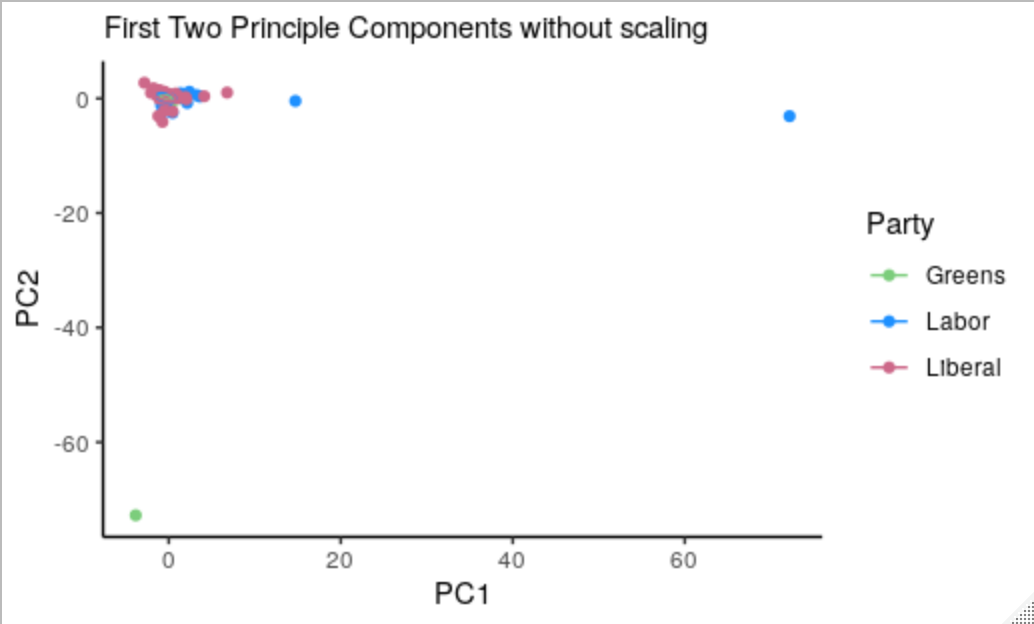
\includegraphics[width=.9\linewidth]{media/20200423103234597_1312556818.png}
\caption{Principlie Comonents with Scaling}
\end{figure}

\begin{HTML}
</p>
\end{HTML}

\begin{HTML}
<!--Newline Important-->
\end{HTML}

\begin{HTML}
</details>
\end{HTML}

\begin{HTML}
<!--Newline Important-->
\end{HTML}

PCA operates by taking a matrix of values, whereby rows are observations
and columns are features, this means we need rows as Documents and
Columns as features in order to perform PCA, this would a be a
DocumentTermMatrix[\textsuperscript{1}].

Geometrically a plot of the first two \emph{Principal Components}
(\(Z_1, Z_2\)) is a projection of data onto the subspace spanned by the
first two loading vectors (\(\phi_1, \phi_2\))

To perform the PCA use the \texttt{prcomp} function:

\begin{verbatim}
  pol.pca <- prcomp(tweet_weighted, scale = FALSE)
\end{verbatim}

This returns a \texttt{prcomp} object that is essentially a list with

\begin{itemize}
\item a \texttt{rotation} matrix

\begin{itemize}
\item (which is a matrix of the loading vectors)
\end{itemize}

\item a matrix of the co-ordinates in the Principle Compenent frame of
reference

\begin{itemize}
\item denoted by \texttt{x}
\end{itemize}

\item \texttt{sdev}; The standard deviation attributable to each principle
component.
\item \texttt{centre} which is a logical indicating whether centring was used

\begin{itemize}
\item If centring was used it will be a vector of the \texttt{centre} values
\end{itemize}

\item \texttt{scale} which is a logical indicating whether scaling was used

\begin{itemize}
\item If scaling was used it will be a vector of the \texttt{scale} values
\end{itemize}
\end{itemize}

\subsubsection{Bi Plot}
\label{sec:orgcd4694d}
a \href{https://en.wikipedia.org/wiki/Biplot}{Biplot} is a plot of the
first two principle components and the corresponding loading vectors.
Roughly speaking, the loading vectors help show the explanation each
variable contributes to a principle component.[\textsuperscript{2}]

\begin{HTML}
<p style=``font-family:Courier New,Courier, monospace,serif;font-size:22px;font-style:italic; '' align=``right'' color=``blue''>
\end{HTML}

\#biplot

\begin{HTML}
</p>
\end{HTML}

A biplot can be produced by simply using the \texttt{biplot} function:

\begin{verbatim}
  biplot(pol.pca, cex = 0.5)
\end{verbatim}

\begin{quote}
See also \href{https://github.com/vqv/ggbiplot}{the ggbiplot package}
\end{quote}

\subsubsection{Scree Plot}
\label{sec:org2cb97db}
A scree plot is a plot of the variance explained by each principle
component, Ideally we would find a vertex where we could cut it off and
say that the data can be explained by said principle components, for
large data sets like this it isn't the case however.

To create a scree plot basically just plot the \texttt{sdev} in as a line or
barchart, just be mindful to encode the names of the \emph{Principal
Components} as ordered factors because otherwise the order may not be
preserved:

\begin{verbatim}
  pcaVar <- pol.pca$sdev ^ 2
  pcaVar <- pcaVar[1:10]
  pcaVarpr <- pcaVar / sum(pcaVar)
  pcaVarpr <- enframe(pcaVarpr)

  names(pcaVarpr) <- c("Principal.Component", "Proportion.Variance")
                          ## This throws a warning
  for (i in 1:nrow(pcaVarpr)) {
    pcaVarpr[["Principal.Component"]][i] <- paste("PC", i)
  }

  pcaVarpr$Principal.Component <-
    factor(
      pcaVarpr$Principal.Component,
      ordered = TRUE,
      levels = pcaVarpr$Principal.Component
    )

  ggplot(data = pcaVarpr,
         aes(x = Principal.Component,
             y = Proportion.Variance,
             group = 1)) +
    geom_point(size = 3, alpha = 0.7, col = "RoyalBlue")  +
    geom_line(col = "IndianRed") +
    labs(x = "Principal Component",
         y = "Proportion of Variance",
         title = "Variance Explained by PC, TF-IDF Weigthing Tweets by Party Leaders") +
    theme_classic() +
    geom_vline(xintercept = 4,
               col = "purple",
               lty = 2)
\end{verbatim}

\begin{figure}[htbp]
\centering
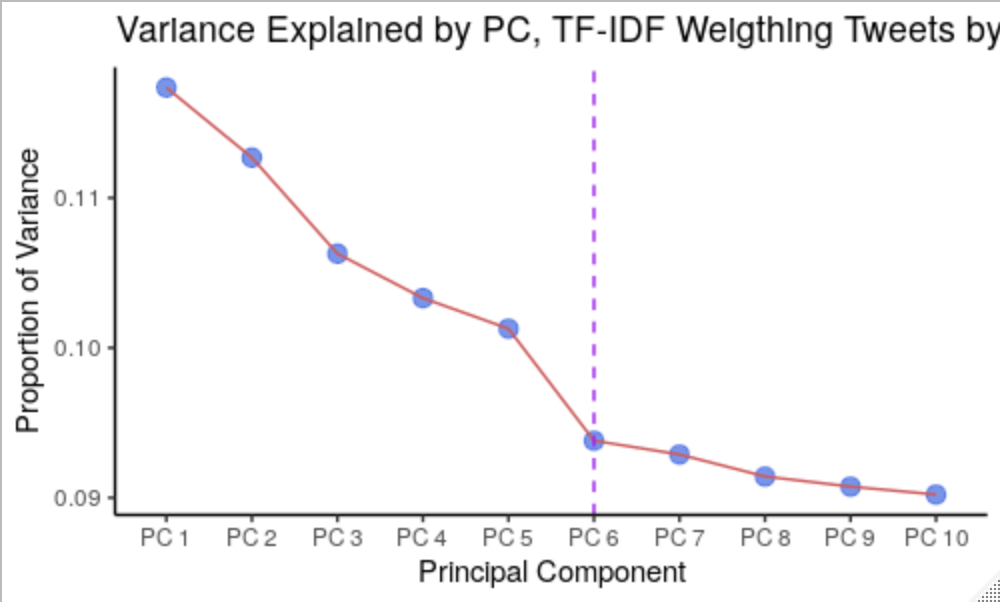
\includegraphics[width=.9\linewidth]{media/20200423115138578_255205396.png}
\caption{Scree Plot of Tweets}
\end{figure}

\subsubsection{Plot the First two PCA's}
\label{sec:org1151b7d}
In order to plot the first two PC's, create a data frame:

\begin{verbatim}
  pca_data$Party  <-
    factor(c(rep("Greens", n), rep("Labor", n), rep("Liberal", n)))
  pol.km <-
    kmeans(tweet_weighted, centers = 3, nstart = 200) %>%  as.vector()
  pca_data$kmeans <- as.factor(pol.km$cluster)
  head(pca_data)
\end{verbatim}

Then it's just a matter of calling ggplot:

\begin{verbatim}
  ggplot(data = pca_data,
         aes(x = PC1, y = PC2, size = PC3, col = Party)) +
    geom_point(alpha = 0.3) +
    ##  geom_point(aes(shape = kmeans)) +
    theme_classic() +
    ## Colours are applied in order of appearance of the factor
    ## Introduce factors alphabetically where possible
    scale_color_manual(values = c("Palegreen3", "DodgerBlue", "Palevioletred3")) +
    scale_size(range = c(0.1, 3)) +
    labs(main = "Tweets by Part Leaders using TF-IDF Weighting",
         subtitle = "First Two Principle Components without scaling") +
    stat_ellipse() ## +
    ## Scaling Fix
    ##  scale_x_continuous(limits = c(-quantile(pca_data$PC1, c(0.99)), quantile(pca_data$PC1, c(0.99)))) +
    ##  scale_y_continuous(limits = c(-quantile(pca_data$PC2, c(0.99)), quantile(pca_data$PC2, c(0.99))))

\end{verbatim}

in this example I encoded the third principle component as the size of
the points:

\begin{figure}[htbp]
\centering
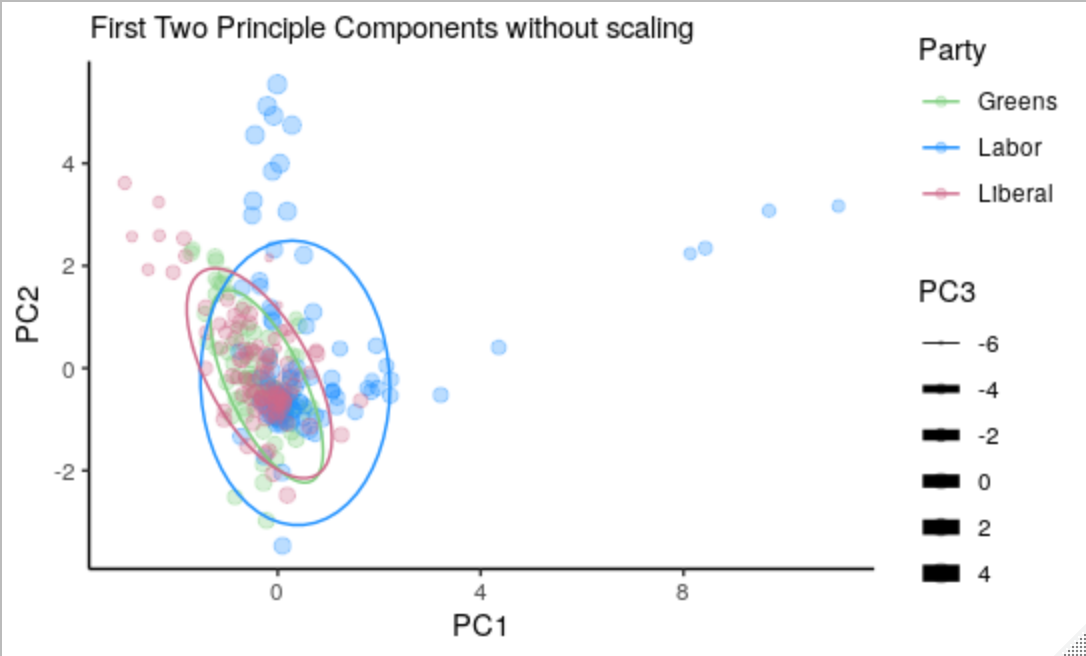
\includegraphics[width=.9\linewidth]{media/20200423115557535_1624578072.png}
\caption{First Two Principle Components}
\end{figure}

\subsection{Use Multi-Dimensional Scaling to Visualise the tweets}
\label{sec:org60f49ca}
The whole idea of Multi-Dimensional Scaling is to \#\#\# Using the \texttt{dist}
function in \textbf{\emph{R}} The \texttt{dist} function takes each row as a vector and
each column as a variable (i.e. axis) of that vector, it then compares
every point and produces a table summarising every combination of
possible differences, so for example the matrix:

\$\$\begin{aligned}
\begin{bmatrix}
  0 & 0 & 5 \\
  0 & 4 & 0 \\
  3 & 0 & 0
\end{bmatrix}
\end{aligned}\$\$

that matrix in \textbf{\emph{R}} would really represent the three vectors
\(\vec{v_1} = \left<0, 0, 3 \right>, \vec{v_2} = \left<0, 4, 0 \right>, \vec{v_3} = \left<5, 0, 0 \right>\)
and so there would be three possible distances we could be possibly be
interested in:

\begin{itemize}
\item \(\left| \left| \vec{v_1} - \vec{v_2} \right| \right| = \left| \left| \vec{v_1} - \vec{v_2} \right| \right|= \mathrm{d}\left( \vec{v_1}, \vec{v_2} \right) = \mathrm{d}\left( \vec{v_2}, \vec{v_1} \right)\)
\item \(\left| \left| \vec{v_1} - \vec{v_3} \right| \right| = \left| \left| \vec{v_3} - \vec{v_1} \right| \right| = \mathrm{d}\left( \vec{v_1}, \vec{v_3} \right) = \mathrm{d}\left( \vec{v_3}, \vec{v_1} \right)\)
\item \(\left| \left| \vec{v_2} - \vec{v_3} \right| \right| = \left| \left| \vec{v_3} - \vec{v_2} \right| \right| = \mathrm{d}\left( \vec{v_2}, \vec{v_3} \right) = \mathrm{d}\left( \vec{v_2}, \vec{v_3} \right)\)
\end{itemize}

\textbf{\emph{R}} will return this as a table (well a \texttt{matrix} class) like this:

\begin{center}
\begin{tabular}{llll}
 & Vector 1 & Vector 2 & Vector 3\\
\hline
Vector 1 & 0 & Repeated & Repeated\\
Vector 2 & \(\mathrm{d}\left(1, 2\right)\) & 0 & Repeated\\
Vector 3 & \(\mathrm{d}\left(1, 2\right)\) & \(\mathrm{d}\left(1, 2\right)\) & 0\\
 &  &  & \\
\end{tabular}
\end{center}

\begin{quote}
\texttt{help(diff)}; This function computes and returns the distance matrix
computed by using the specified distance measure to compute the
distances between the rows of a data matrix.
\end{quote}

So if we did this all in \textbf{\emph{R}} with some arbitrary numbers:

\begin{verbatim}
  (rbind(c("x" = 0, "y" = 0, "z" = 4),
        c("x" = 1, "y" = 1, "z" = 1),
        c("x" = 0, "y" = 3, "z" = 0))) %>% dist()
\end{verbatim}

\begin{verbatim}
       x y z
  [1,] 0 0 4
  [2,] 1 1 1
  [3,] 0 3 0
  >
           1        2
  2 3.316625
  3 5.000000 2.449490
\end{verbatim}

Then we could use this distances to visualise these vectors by plotting
them in such a way that preserves the distances, in order to do that the
\texttt{cmdscale} can be used:

\begin{quote}
\texttt{help(cmdscale)}; Multidimensional scaling takes a set of
dissimilarities and returns a set of points such that the distances
between the points are approximately equal to the dissimilarities. (It
is a major part of what ecologists call 'ordination'.)

A set of Euclidean distances on n points can be represented exactly in
at most \(n - 1\) dimensions. \texttt{cmdscale} follows the analysis of
\href{https://www.tandfonline.com/doi/abs/10.1080/03610927808827707}{Mardia
(1978)}, and returns the best-fitting \$k\$-dimensional representation,
where \(k\) may be less than the argument \texttt{k}. [[][]]

\ldots{} The configuration returned is given in principal-component axes\ldots{}
\end{quote}

\subsubsection{Finding the Distance Matrix of Tweets}
\label{sec:orgefc6573}
In order to find the distance matrix of the tweets first be mindful that
the matrix must have rows as observations and columns as features, then
it's just a matter of calling \texttt{dist} over the matrix, in order to
producs the \emph{Classical Multidimensional Scaling} representation, simply
pass this distance matrix to the \texttt{cmdscale} function and it will do all
the work:

\begin{verbatim}
  tweet_matrix[1:3, 1:3]
  tweet_dist <- dist(tweet_weighted)
  tweet_mds  <- cmdscale(d = tweet_dist, k = 2)
  tweet_mds.df <- as.data.frame(tweet_mds)
  names(tweet_mds.df) <- c("MDX", "MDY")
  head(tweet_mds.df)

  ## Add Colours
  tweet_mds.df$Party <- factor(c(rep("Greens", n), rep("Labor", n), rep("Liberal", n)))
\end{verbatim}

which will produce a data frame like this:

\begin{verbatim}
       MDX    MDY Party
     <dbl>  <dbl> <fct>
  1 -0.427  0.211 Greens
  2 -0.447  0.294 Greens
  3 -0.240 -0.320 Greens
  4 -0.541  0.249 Greens
  5 -0.302  0.374 Greens
  6 -0.388 -0.278 Greens
\end{verbatim}

Then it's simply a matter of plotting it which is easy enough:

\begin{verbatim}
  (ggmds <- ggplot(mds_data, aes(x = MDX, y = MDY, col = Party)) +
    geom_point() +
    scale_color_manual(values = c("Palegreen3", "DodgerBlue", "Palevioletred3")) +
    theme_classic())
\end{verbatim}

\begin{figure}[htbp]
\centering
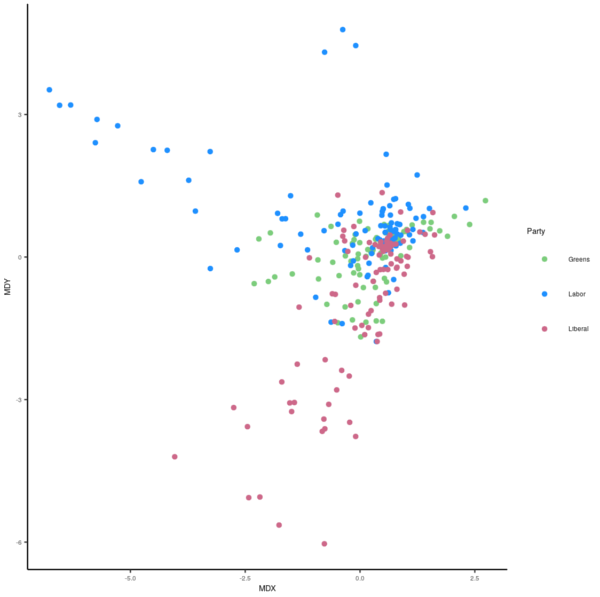
\includegraphics[width=.9\linewidth]{media/20200426094721532_1205049402.png}
\caption{MDS Plot of Party Tweets, Euclidean 2dim}
\end{figure}

\subsubsection{Binary Distance}
\label{sec:org132f928}
In much the same way binary distance could be plotted by specifying that
particular method (without the niceties of \texttt{ggplot}):

\begin{verbatim}
  # Binary Distance ==============================================================
  ## Remember to use the weigted values though,
  ## The weighted values are a good adjustment and is consistent with different
  ## measures of distance
  dist_mat_bin <- dist(tweet_matrix, method = "binary")
  mds_data_bin <- cmdscale(dist_mat_bin, k = 2)
  plot(mds_data_bin[,1], mds_data_bin[,2], col = c("ForestGreen", "PowderBlue", "MediumVioletRed")[pca_data$Party])
\end{verbatim}

\subsubsection{Cosine Distance}
\label{sec:orgbab8904}
\begin{enumerate}
\item Finding Unit Vectors
\label{sec:org54c7dde}
Recall that taking the matrix multiplication of a diagonal matrix is
equivalent to multipling each term of a matrix by a value, for example:

\$\$
\left(
\begin{array}{ccc}
 a_{1,1} & a_{1,2} & a_{1,3} \\
 a_{2,1} & a_{2,2} & a_{2,3} \\
 a_{3,1} & a_{3,2} & a_{3,3} \\
\end{array}
\right) \(\cdot\)
\left(
\begin{array}{ccc}
 b_1 & 0 & 0 \\
 0 & b_2 & 0 \\
 0 & 0 & b_3 \\
\end{array}
\right) =
\left(
\begin{array}{ccc}
 b_1 a_{1,1} & b_2 a_{1,2} & b_3 a_{1,3} \\
 b_1 a_{2,1} & b_2 a_{2,2} & b_3 a_{2,3} \\
 b_1 a_{3,1} & b_2 a_{3,2} & b_3 a_{3,3} \\
\end{array}
\right)
\$\$

Play around this in \emph{Wolfram Mathematica}:

\begin{verbatim}
  Aeg = Array[Subscript[a, #1, #2] &, {3, 3}];
  Aeg // MatrixForm
  Beg = {Subscript[b, 1], Subscript[b, 2], Subscript[b, 3]} //
    DiagonalMatrix
  (Aeg.Beg) // MatrixForm
\end{verbatim}

So in order to create a vector of unit vectors it is sufficient to
merely perform:

\begin{verbatim}
  U   <- tweet_matrix %*% diag(1/sqrt(colSums(tweet_matrix^2)))
  U_w <- tweet_weighted %*% diag(1/sqrt(colSums(tweet_weighted^2)))
\end{verbatim}

\item Vector Dot Product
\label{sec:org70ac74d}
The dot product of two vectors is the area spanned by a rectangle of
length equal to the first vector and width equal to the projection
(i.e. the shadow) of the first vector onto the second.

The cosine similarity is the length of that projection, if the length of
both vectors are independetly scaled to one, the dot product will be
different but the angle won't change, also the area of the dot product
will be \(1 \times\) the projection:

$$\begin{aligned}
    \left| \left| \mathbf{X} \right| \right| = \left|  \left| \mathbf{Y} \right| \right|  &\implies   \frac{\mathbf{\mathbf{X}\cdot  \mathbf{Y}}}{\left| \left| \mathbf{X} \right| \right|\times \left| \left| \mathbf{Y} \right| \right|}\\
    &= \mathbf{X}\cdot  \mathbf{Y} \\
    &= \cos\left( \mathbf{X}, \mathbf{Y} \right)\\
    &= \sum^{n}_{i= 1}   \left[ x_i y_i \right]
\end{aligned}$$

Hence the \href{https://en.wikipedia.org/wiki/Euclidean\_distance}{Euclidean
Distance} will be:

$$\begin{aligned}
\mathrm{dist}\left( \mathbf{X}, \mathbf{Y} \right)= \left| \left| \mathbf{X}-\mathbf{Y} \right| \right| \\
&= \sqrt{\sum^{n}_{i= 1}   \left[ \left( x_i-y_i \right)^2 \right] } \\
\mathrm{dist}\left( \mathbf{X}, \mathbf{Y} \right)^2&= \sum^{n}_{i= 1}  \left[ \left( x_i-y_i \right)^2 \right] \\
&= \sum^{n}_{i= 1}   \left( x^2 \right)+  \sum^{n}_{i= 1}   \left( y_i^2 \right)+ 2 \sum^{n}_{i= 1}   \left( x_iy_i \right) \\
&= 1+ 1 +  2 \times  \frac{\sum^{n}_{i= 1}   \left( x_iy_i \right)}{\left( 1 \right) }\\
&= 2+ 2\times \frac{\sum^{n}_{i= 1}   \left( x_iy_i \right)}{\left| \left| \mathbf{X} \right| \right|\times \left| \left| \mathbf{Y} \right| \right|}\\
&= 2+ 2 \cos\left( \mathbf{X}, \mathbf{Y} \right)\\
\ \\
& \implies  \left( 1- \cos\left( \mathbf{X}, \mathbf{Y} \right) \right) = \frac{\mathrm{dist}\left( \mathbf{X}, \mathbf{Y} \right)}{2}
\end{aligned}$$

The only thinig to note is that the cosine similarity is 1 when two
vectors are identical in direction but is 0 when they are totally
different in direction (i.e. perpendicular or rather orthogonal). For a
metric of distance we want it the other way around so we just subtract
it from 1.

So in order to determine the cosine distance, it is sufficient to
perform the following:

\begin{verbatim}
   # Cosine Distance===============================================================
  # Create Unit Vectors ##########################################################
  ## Recall matrix multiplication of a diagonalised matrix is product of elements
  U   <- tweet_matrix %*% diag(1/sqrt(colSums(tweet_matrix^2)))
  U_w <- tweet_weighted %*% diag(1/sqrt(colSums(tweet_weighted^2)))
  # Create Distance Matrix #######################################################
  # Plot the MDS #################################################################
  ## Make the Distance Matrix
  dist_mat_cos <-dist(U_w, method = "euclidean")^2/2
  ## Make the MDS
  mds_data_cos <- cmdscale(dist_mat_cos, k = 2)
  names(mds_data_cos) <- c("xvals", "yvals")
  plot(mds_data_cos[,1], mds_data_cos[,2], col = pca_data$Party)
\end{verbatim}

which will produce something like this:

\begin{center}
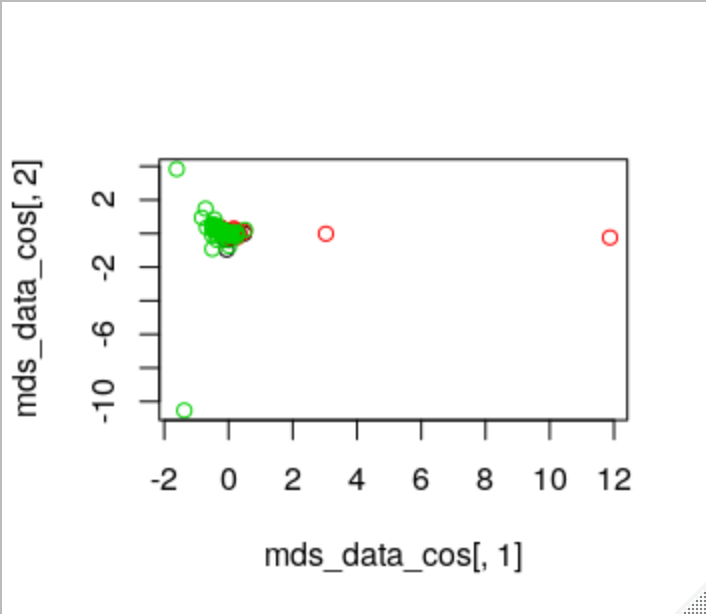
\includegraphics[width=.9\linewidth]{./media/20200426101157206_1262456543.png}
\end{center}

This was converted from `md` to `org` using `pandoc -f gfm` at time:
2020-04-26T01-57-51
\end{enumerate}
\end{document}
